\section{Synchronizing Shapes with \prism}
\label{sec:prism}

\td{Mention the role of identity preservation somewhere, and why we exchange IDs in the patches}

\Cref{fig:prism} depicts our prototype approach to the problem of synchronizing shapes of a language, \prism.
The key idea is that every change occuring on one incarnation is shipped to all other incarnations of the same model in the form of a \patch.
\prism keeps track of a matrix that associates every ``conceptual'' model to its incarnations in various LVs.
When a change occurs on one incarnation, as the result of a user edit or following an execution step of an interpreter, for instance, the LV hosting this incarnation generates a \patch describing the change as a set of CRUD-like operations.
In our prototype implementation, the structure of this patch is prescribed by the Rascal ADT shown in \Cref{lst:delta-adt}, largely inspired by the ``edit scripts'' proposed by \citeauthor{rozen2017towards}~\cite{rozen2017towards}.
Essentially, patches consist of a set of operations attached to particular elements of the model.

%On the edition of an incarnation of a model, its containing LV creates a patch describing the changes. The LV ships the patch to \prism, which then propagates the patch to every other incarnation of the same model. \prism use a simple matrix that keeps track of the associations between models and their incarnations in various LVs.
%Every LV is then responsible for updating its own incarnation by interpreting the patch.

\begin{figure}[bt]
	\centering
	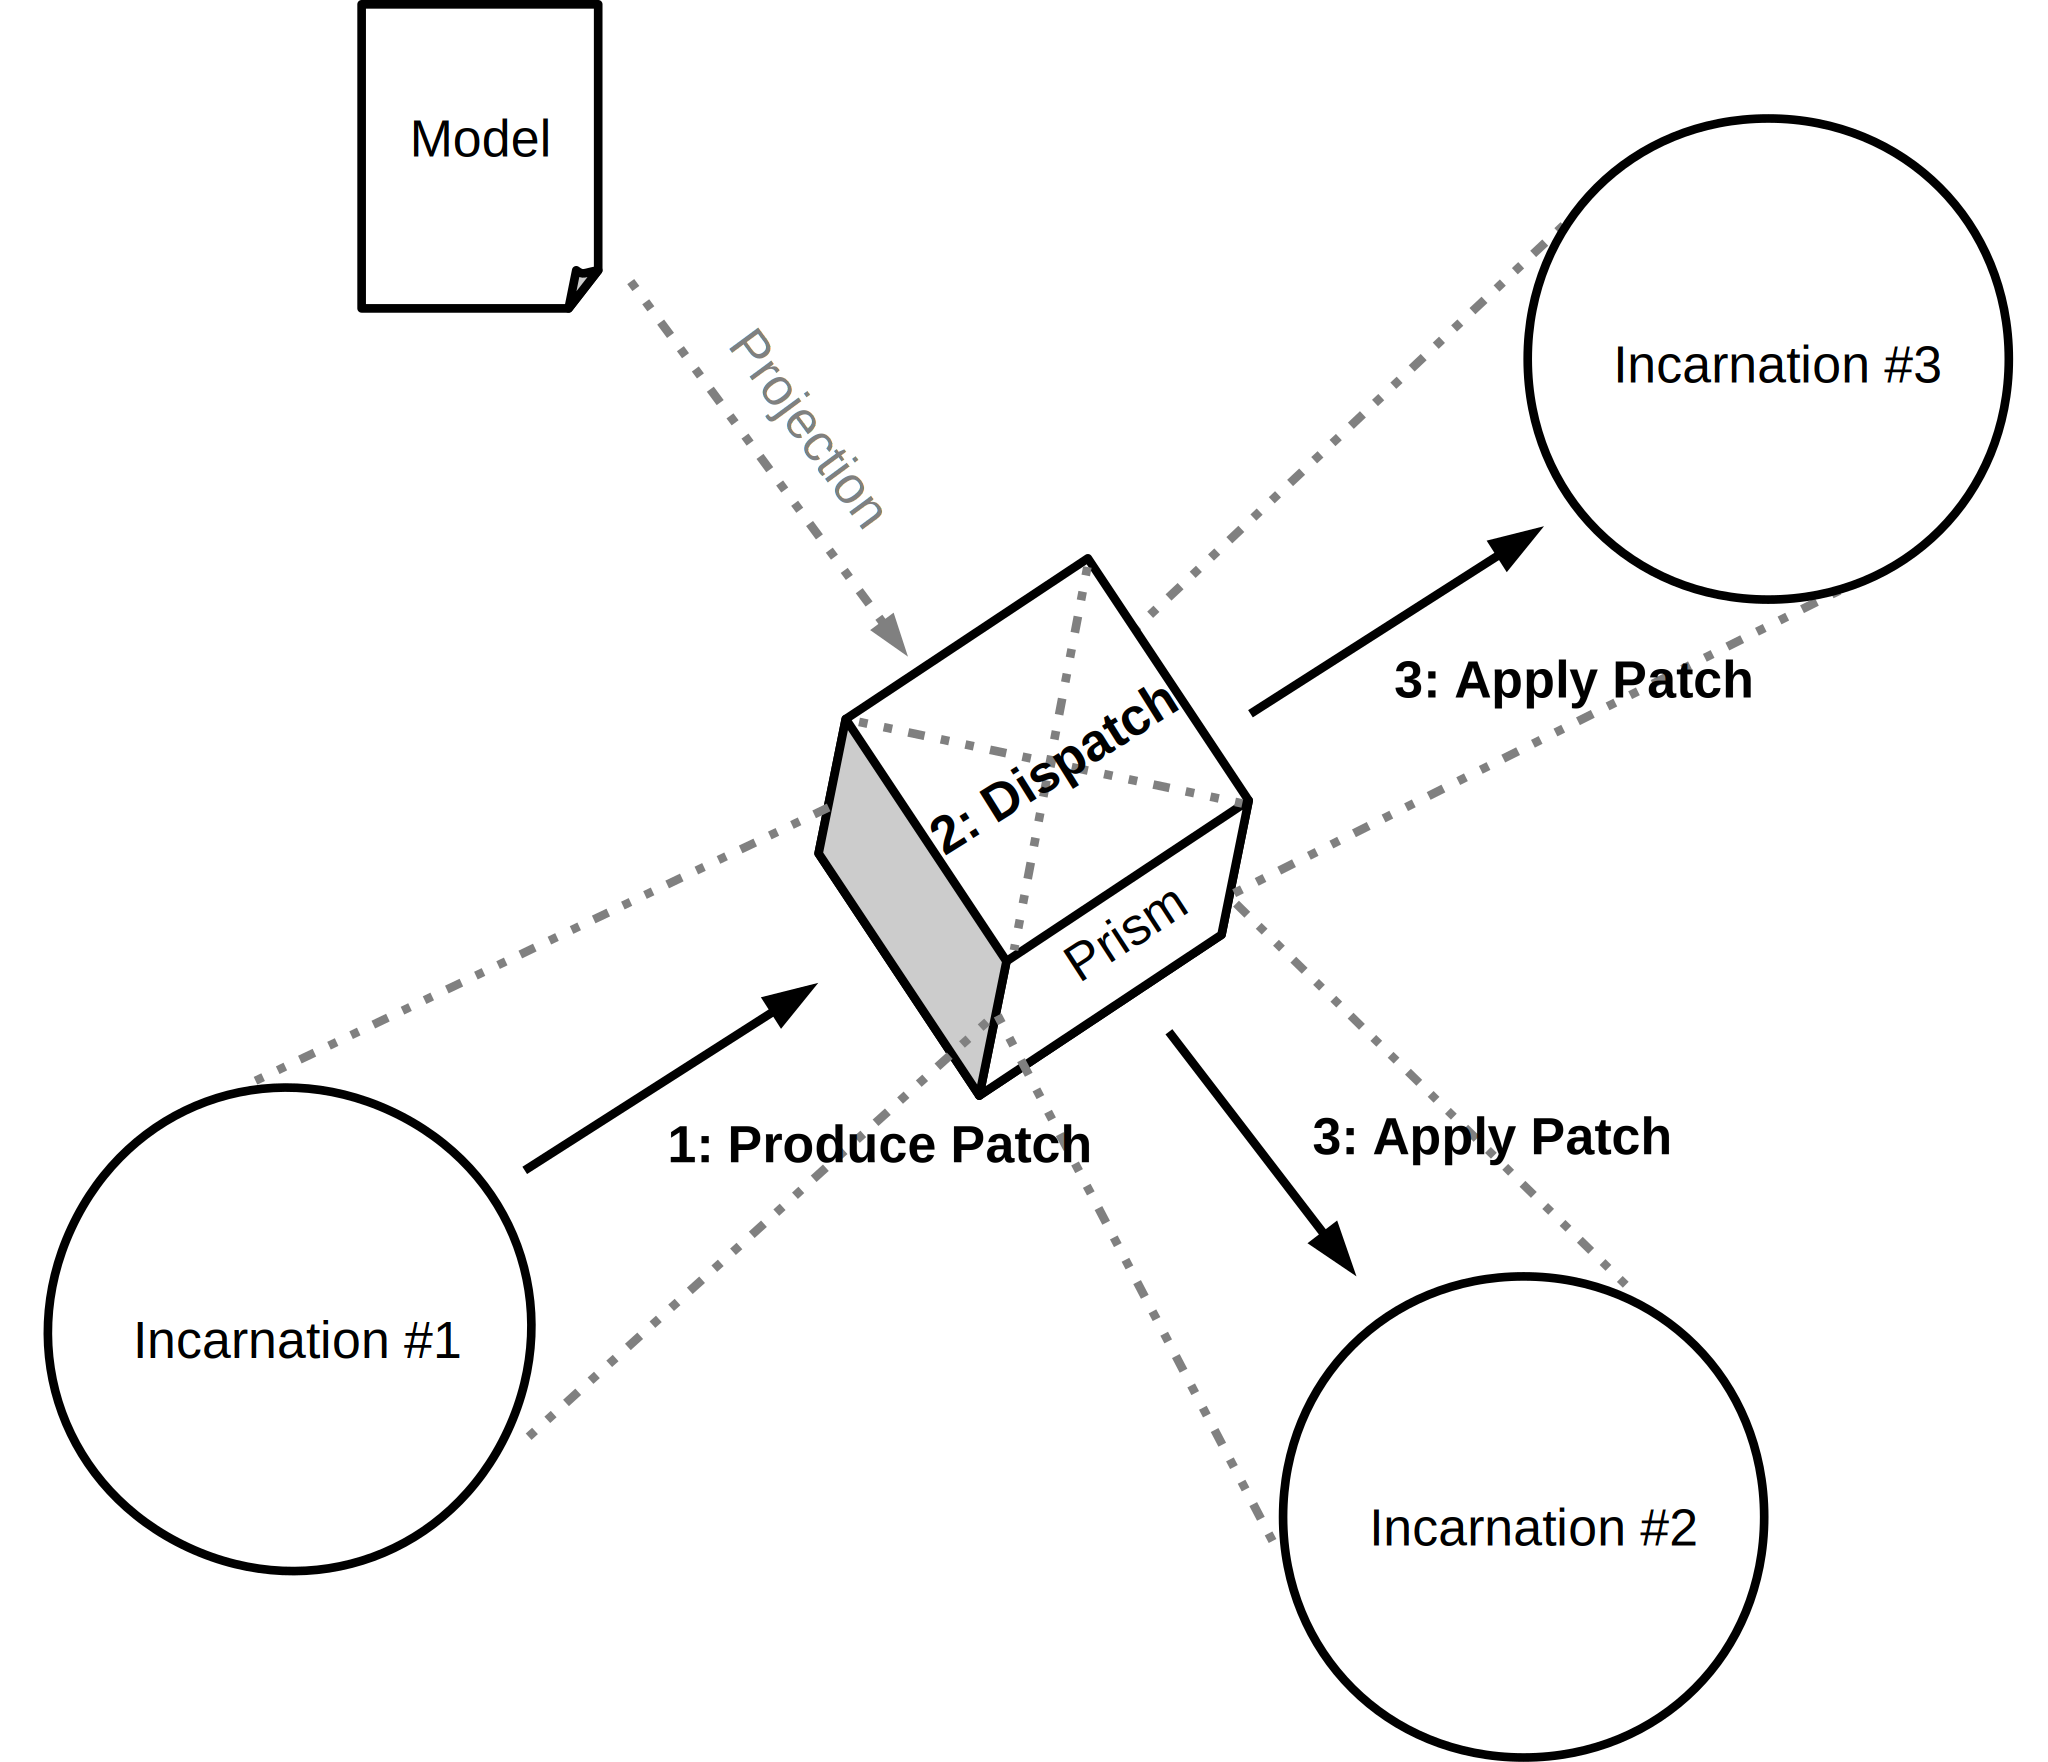
\includegraphics[width=.6\columnwidth]{figures/prism}
	\caption{Using \prism to synchronize three incarnations of the same model. Here, a change occurs on Incarnation \#1 and the resulting patch is dispatched to Incarnation \#2 and \#3.}
	\label{fig:prism}
\end{figure}

Our approach keeps the LV fully independent and builds a communication bus between them.
Both representations of the same model in various LV are kept in memory to allow online synchronization of the same models manipulated by different stakeholders in different shapes.
When a changes occurs on either side, this LV is responsible for generating a \emph{patch} (aka. \de or edit script~\cite{rozen2017towards}), that stores the changes on the model that have been realized on this LV.
The communication bus then ships this patch to all the other LVs.
Every LV interprets the patch in its own way to keep the representation synchronized.
On the EMF LV, for instance, the patch is interpreted as a set of changes that impact an Ecore model, while on the Rascal LV it is interpreted as a set of changes that impact a value conforming to the ADT defining the AS of the language.

It is important to note that each LV may want to preserve certain information across the patches that are specific to the LV.
A textual editor in Rascal, for instance, needs to keep some of the parsing information to maintain layout whenever patches are applied.
So it should be possible to apply the patch while maintaining the extra information specific to a given LV.
Intuitively, our approach supposes that all the information that does not relate to the constructs of a language is ``extra'' and therefore escape the synchronization. \td{FIXME}

Automatically generating language implementations in different LV is beyond the scope of this paper.
Instead, given various shapes of a language, implemented by hand, we provide the means to automatically synchronize the projections of a model.

\td{Write a paragraph on ``connecting a LV $\Leftrightarrow$ implementing produce/apply patch''}
\td{+ a paragraph on what does the dispatch do \emph{exactly}: no parallel edits, \etc}
\td{Highlight incrementality, \ie~we're not Xtext, $\neq$ full de-/re-serialization}

\begin{lstlisting}[label=lst:delta-adt, caption={CRUD-like patch definition in Rascal}, language=Rascal, float=tb]
@doc{A patch consists of a sequence of edits}
alias Patch = tuple[Id root, Edits edits];

@doc{Edits are operations attached to object identities}
alias Edits = lrel[Id obj, Edit edit];

data Edit
  = put(str field, value val)
  | unset(str field)
  | ins(str field, int pos, value val)
  | del(str field, int pos)
  | create(str class) 
  | destroy();
\end{lstlisting}

It is important to note that ``projections'' have no relation whatsoever with projectional editing.
A projection denotes the incarnation of a model in a particular shape of a language.
In \Cref{fig:motivating-fsm}, the lower part depicts three projections of the same \texttt{Button} state machine model in three shapes of the FSM language.
We use the term ``language'' to refer to the specification of a language independently from its realization in a given LV.
A concrete implementation of a language is a ``shape''.
An instance of a shape, \ie~a particular model in a particular LV, is a ``projection'' of a ``virtual'' model.
Metamorphic synchronization refers to the ability to synchronize the projections of a given model for every shapes of a language.
